\documentclass[12pt, titlepage]{article}

\usepackage{fullpage}
\usepackage[round]{natbib}
\usepackage{multirow}
\usepackage{booktabs}
\usepackage{tabularx}
\usepackage{graphicx}
\usepackage{xcolor}
\usepackage{url}
\usepackage{caption}
%\usepackage{geometry}

\usepackage{xr}
\usepackage{hyperref}
\usepackage[numbib,nottoc]{tocbibind}

\hypersetup{
 bookmarks=true,   % show bookmarks bar?
 colorlinks=true,  % false: boxed links; true: coloured links
 linkcolor=red,   % color of internal links (change box color 
%with linkbordercolor)
 citecolor=black!40,  % color of links to bibliography
 filecolor=magenta,  % color of file links
 urlcolor=cyan   % color of external links
}

%% Comments

\usepackage{color}

\newif\ifcomments\commentstrue

\ifcomments
\newcommand{\authornote}[3]{\textcolor{#1}{[#3 ---#2]}}
\newcommand{\todo}[1]{\textcolor{red}{[TODO: #1]}}
\else
\newcommand{\authornote}[3]{}
\newcommand{\todo}[1]{}
\fi

\newcommand{\wss}[1]{\authornote{blue}{SS}{#1}}
\newcommand{\an}[1]{\authornote{magenta}{Author}{#1}}


\newcommand{\progname}{SSP}

\newcounter{acnum}
\newcommand{\actheacnum}{AC\theacnum}
\newcommand{\acref}[1]{AC\ref{#1}}

\newcounter{ucnum}
\newcommand{\uctheucnum}{UC\theucnum}
\newcommand{\uref}[1]{UC\ref{#1}}

\newcommand{\rref}[1]{R\ref{#1}}

\newcounter{mnum}
\newcommand{\mthemnum}{M\themnum}
\newcommand{\mref}[1]{M\ref{#1}}

%\newgeometry{margin=2cm}

% define "struts", as suggested by Claudio Beccari in
%    a piece in TeX and TUG News, Vol. 2, 1993.
\newcommand{\Tstrut}{\rule{0pt}{2.6ex}}         % = `top' strut

\externaldocument[SRS-]{../../SRS/SRS}
\externaldocument[MIS-]{MIS_SSP}

\begin{document}

\title{Module Guide for Slope Stability Analysis Program} 
\author{Henry Frankis and Brooks MacLachlan}
\date{\today}

\maketitle

\pagenumbering{roman}

\section{Revision History}

\begin{tabularx}{\textwidth}{p{3cm}p{2cm}X}
	\toprule {\bf Date} & {\bf Version} & {\bf Notes}\\
	\midrule
	31/10/2018 & 1.0 & Initial template and module updates\\
	11/01/2018 & 1.1 & Anticipated changes updates\\
	\bottomrule
\end{tabularx}

\newpage

\section{Reference Material}
This section records information for easy reference.
\subsection{Abbreviations and Acronyms}

\renewcommand{\arraystretch}{1.2}
\begin{tabular}{l l} 
	\toprule		
	\textbf{Symbol} & \textbf{Description}\\
	\midrule 
	AC & Anticipated Change\\
	DAG & Directed Acyclic Graph \\
	M & Module \\
	MG & Module Guide \\
	OS & Operating System \\
	R & Requirement\\
	SC & Scientific Computing \\
	SRS & Software Requirements Specification\\
	\progname & Slope Stability Analysis Program\\
	UC & Unlikely Change \\
	\bottomrule
\end{tabular}\\

\bmac{This section is not on the template but I think that it should be since 
this document introduces many new acronyms}

\newpage

\tableofcontents

\listoftables

\listoffigures

\newpage

\pagenumbering{arabic}

\section{Introduction}

\hspace{3ex}Decomposing a system into modules is a commonly accepted
approach to developing software.  A module is a work assignment for a
programmer or programming team~\citep{ParnasEtAl1984}.  In the best
practices for Scientific Computing (SC), \citet{WilsonEtAl2013} advise a
modular design, but are silent on the criteria to use to decompose the
software into modules.  We advocate a decomposition based on the
principle of information hiding~\citep{Parnas1972a}.  This principle
supports design for change, because the ``secrets'' that each module
hides represent likely future changes.  Design for change is valuable
in SC, where modifications are frequent, especially during initial
development as the solution space is explored.

Our design follows the rules laid out by \citet{ParnasEtAl1984}, as follows:
\begin{itemize}  
\item System details that are likely to change independently should be
  the secrets of separate modules.
\item Any other program that requires information stored in a module's
  data structures must obtain it by calling access programs belonging
  to that module.
\end{itemize}

\bmac{There is an item here in the template saying "each data structure is used 
in only one module", which just seems wrong to me. Maybe each data structure is 
implemented by a dedicated module, but then many other modules can still use 
that data structure (module).}

In a rational design process, the Module Guide (MG) is developed after 
completing the Software Requirements Specification (SRS) 
\citep{ParnasEtAl1984}. The MG specifies the modular
structure of the system and is intended to allow both designers and
maintainers to easily identify the parts of the software.  The
potential readers of this document are as follows:

\begin{itemize}
\item New project members: This document can be a guide for a new
  project member to easily understand the overall structure and
  quickly find the relevant modules they are searching for.
\item Maintainers: The hierarchical structure of the module guide
  improves the maintainers' understanding when they need to make
  changes to the system. It is important for a maintainer to update
  the relevant sections of the document after changes have been made.
\item Designers: Once the module guide has been written, it can be
  used to check for consistency, feasibility, and flexibility. Designers can 
  verify the system in various ways, such as consistency among modules, 
  feasibility of the decomposition, and flexibility of the design.
\end{itemize}

The rest of the document is organized as follows. Section
\ref{SecChange} lists the anticipated and unlikely changes of the
software requirements. Section \ref{SecMH} summarizes the module
decomposition that was constructed according to the likely
changes. Section \ref{SecConnection} specifies the connections between
the software requirements and the modules. Section \ref{SecMD} gives a
detailed description of the modules. Section \ref{SecTM} includes two
traceability matrices. One checks the completeness of the design
against the requirements provided in the SRS. The other shows the
relation between anticipated changes and the modules. Section
\ref{SecUse} describes the use relation between modules.

\section{Anticipated and Unlikely Changes} \label{SecChange}

\hspace{3ex}This section lists possible changes to the
system. According to the likeliness of the change, the possible
changes are classified into two categories. Each Anticipated Change (AC) is
listed in Section \ref{SecAchange}, and each Unlikely Change (UC) is listed in
Section \ref{SecUchange}.

\subsection{Anticipated Changes} \label{SecAchange}

\hspace{3ex}Anticipated changes are the source of the information that
is to be hidden inside the modules. Ideally, changing one of the
anticipated changes will only require changing the one module that
hides the associated decision. The approach adapted here is called
design for change.

\begin{description}
\item[AC\refstepcounter{acnum}\theacnum \label{AC_hardware}:] The
  specific hardware on which the software is running.
\item[AC\refstepcounter{acnum}\theacnum \label{AC_Control}:] The
  algorithm for the overall operation procedure of the program.
\item[AC\refstepcounter{acnum}\theacnum \label{AC_input}:] The format
  of the initial input data.
\item[AC\refstepcounter{acnum}\theacnum \label{AC_output}:] The format
  of the final output data.
\item[AC\refstepcounter{acnum}\theacnum \label{AC_GenAlg}:] Algorithm
  for determining the critical slip surface.
\item[AC\refstepcounter{acnum}\theacnum \label{AC_Kin}:] Criteria for
  a slip surface to be considered physically realistic.
\item[AC\refstepcounter{acnum}\theacnum \label{AC_FSweight}:] The
  weighting scheme for comparing slip surfaces factors of safety.
\newline\bmac{AC5-AC7 are all related to the genetic algorithm}
\item[AC\refstepcounter{acnum}\theacnum \label{AC_Slicer}:] The
  algorithm for dividing a slip surface into slices.
\item[AC\refstepcounter{acnum}\theacnum \label{AC_MP}:] The
  algorithm for implementation of the Morgenstern-Price method.
\item[AC\refstepcounter{acnum}\theacnum \label{AC_PropSorter}:] The
  algorithm for calculating soil properties of and forces on slices.
\newline\bmac{AC8-AC10 are all related to the Morgenstern-Price method}
\item[AC\refstepcounter{acnum}\theacnum \label{AC_Array}:] The
  implementation for the sequence (array) data structure.
\item[AC\refstepcounter{acnum}\theacnum \label{AC_Rand}:] The method
  of generating pseudo-random numbers.
\newline\bmac{Also related to genetic algorithm}
\item[AC\refstepcounter{acnum}\theacnum \label{AC_Plot}:] The method
  for creating plots.
\end{description}


\subsection{Unlikely Changes} \label{SecUchange}

\hspace{3ex}The module design should be as general as
possible. However, a general system is more complex. Sometimes this
complexity is not necessary. Fixing some design decisions at the
system architecture stage can simplify the software design. If these
decision should later need to be changed, then many parts of the
design will potentially need to be modified. Hence, it is not intended
that these decisions will be changed.

\begin{description}
\item [\refstepcounter{ucnum}UC\theucnum \label{UC_IO}:] Input/Output
  devices (Input: File and/or keyboard, Output: File, memory, and/or
  screen).
\item [\refstepcounter{ucnum}UC\theucnum \label{UC_SSPGoal}:] The goals of 
\progname{}, to determine a slope's critical slip surface and corresponding 
factor of safety, will not change.
 
\end{description}


\section{Module Hierarchy} \label{SecMH}

\hspace{3ex}This section provides an overview of the module
design. Modules are summarized in a hierarchy decomposed by secrets
in Table~\ref{Table:Decomp}. The modules listed below are the modules
that will actually be implemented. Modules are numbered by \textbf{M}
followed by a number.

\begin{description}
\item [\refstepcounter{mnum} \mthemnum \label{mHH}:] Hardware-Hiding
\item [\refstepcounter{mnum} \mthemnum \label{mControl}:] Control
\item [\refstepcounter{mnum} \mthemnum \label{mInput}:] Input
\item [\refstepcounter{mnum} \mthemnum \label{mOutput}:] Output
\item [\refstepcounter{mnum} \mthemnum \label{mGenAlg}:] Genetic
  Algorithm
\item [\refstepcounter{mnum} \mthemnum \label{mKinAdm}:] Kinematic
  Admissibility
\item [\refstepcounter{mnum} \mthemnum \label{mSlipWeight}:] Slip Weighting
\item [\refstepcounter{mnum} \mthemnum \label{mSlipSlicer}:] Slip Slicing
\item [\refstepcounter{mnum} \mthemnum \label{mMorgPrice}:]
  Morgenstern-Price Calculation
\item [\refstepcounter{mnum} \mthemnum \label{mSliceProperty}:] Slice
  Property Calculation
\item [\refstepcounter{mnum} \mthemnum \label{mArrayOps}:] Array Data Structure
\item [\refstepcounter{mnum} \mthemnum \label{mRandNum}:] Random Number     
Generation
\item [\refstepcounter{mnum} \mthemnum \label{mPlot}:] Plotting
\end{description}

Note that \mref{mHH} is a commonly used module and is already
implemented by the operating system.

\begin{table}[h!]
\centering
\begin{tabular}{p{0.3\textwidth} p{0.6\textwidth} }
\toprule
\textbf{Level 1} & \textbf{Level 2} \\
\midrule

{Hardware-Hiding} & ~ \\
\midrule

\multirow{8}{0.3\textwidth}{Behaviour-Hiding} &
Control \\
& Input \\
& Output \\
& Genetic Algorithm \\
& Kinematic Admissibility \\
& Slip Weighting \\
& Slip Slicing \\
& Morgenstern Price Calculation \\
& Slice Property Calculation \\
\midrule

\multirow{3}{0.3\textwidth}{Software Decision} &
Array Data Structure \\
& Random Number Generation \\
& Plotting \\
\bottomrule

\end{tabular}
\caption{Module Hierarchy}
\label{Table:Decomp}
\end{table}

\section{Connection Between Requirements and Design} \label{SecConnection}

\hspace{3ex}The design of the system is intended to satisfy the
requirements developed in the SRS. In this stage, the system is
decomposed into modules. The connection between requirements and
modules is listed in Table~\ref{Table:Req}. The program uses the 
Morgenstern-Price method to calculate the factor of safety, which is implemented
by \mref{mMorgPrice}. Further information on the Morgenstern Price algorithm 
can be found in \cite{ZhuEtAl2005}. A genetic algorithm is used to generate 
potential slip surfaces to compare to find the critical slip surface, 
implemented in \mref{mGenAlg}. Further information on use of a genetic 
algorithm in relation to a slope stability problem can be found in 
\cite{LiEtAl}.


\section{Module Decomposition} \label{SecMD}

\hspace{3ex}Modules are decomposed according to the principle of
``information hiding'' proposed by \citet{ParnasEtAl1984}. The
\emph{Secrets} field in a module decomposition is a brief statement of
the design decision hidden by the module. The \emph{Services} field
specifies \emph{what} the module will do without documenting
\emph{how} to do it. For each module, a suggestion for the
implementing software is given under the \emph{Implemented By}
title. If the entry is \emph{OS}, this means that the module is
provided by the operating system or by standard programming language
libraries. If the entry is \emph{\progname}, the module will be implemented by 
\progname. Only the leaf modules in the hierarchy have to be implemented. If a 
dash (\emph{--}) is shown, this means that the module is not a leaf and will 
not have to be implemented. Whether or not this module is implemented depends 
on the programming language selected.

\subsection{Hardware-Hiding (\mref{mHH})}

\begin{description}
\item[Secrets:]The data structure and algorithm used to implement the
  virtual hardware.
\item[Services:]Serves as a virtual hardware used by the rest of the
  system. This module provides the interface between the hardware and
  the software. So, the system can use it to display outputs or to
  accept inputs.
\item[Implemented By:] OS
\end{description}

\subsection{Behaviour-Hiding}

\begin{description}
\item[Secrets:]The contents of the required behaviors.
\item[Services:]Includes programs that provide externally visible
  behaviors of the system as specified in the software requirements
  specification (SRS) documents. This module serves as a communication
  layer between the hardware-hiding module and the software decision
  module. The programs in this module will need to change if there are
  changes in the SRS.
\item[Implemented By:] --
\end{description}

\subsubsection{Control (\mref{mControl})}

\begin{description}
\item[Secrets:] The algorithm for coordinating how the program runs.
\item[Services:] Drives the program through the required tasks.
\item[Implemented By:] \progname
\end{description}


\subsubsection{Input (\mref{mInput})}

\begin{description}
\item[Secrets:]The format and structure of the input data.
\item[Services:] Read, verify, and store the input data. This includes a set of 
  coordinates for each slope layer, soil properties for each layer, 
  specifically effective angle of friction, effective cohesion, dry unit 
  weight, and saturated unit weight, and the coordinates and unit weight of 
  water for a water table, if one exists. This also includes an expected range 
  for the start and end points of the critical slip surface and a decision on 
  whether to use a half-sine or the constant 1 for the interslice normal to 
  shear force ratio variability function.
\item[Implemented By:] \progname
\end{description}

\subsubsection{Output Format (\mref{mOutput})}

\begin{description}
\item[Secrets:] The format and structure of the output data.
\item[Services:] Outputs the results of the calculations, including
  the factor of safety for the critical slip calculated by the
  Morgenstern Price Module (\mref{mMorgPrice}) and a plot of the critical
  slip surface on the slope geometry. Verifies that the output meets physical 
  constraints. Also outputs input values.
\item[Implemented By:] \progname
\end{description} 


\subsubsection{Genetic Algorithm (\mref{mGenAlg})}

\begin{description}
\item[Secrets:] Algorithm for identifying the critical slip surface with the 
minimum factor of safety.
\item[Services:] Generates a set of potential slip surfaces and searches the 
set for the critical slip surface with the minimum factor of safety.
\item[Implemented By:] \progname
\end{description}


\subsubsection{Kinematic Admissibility (\mref{mKinAdm})}

\begin{description}
\item[Secrets:] The kinematic admissibility criteria for determining if a given 
slip surface is realistic physically.
\item[Services:] Tests slip surfaces for physically unlikely features including 
sharp angles, points outside of the soil bed, or downward concavity.
\item[Implemented By:] \progname
\end{description} 

\subsubsection{Slip Weighting (\mref{mSlipWeight})}

\begin{description}
\item[Secrets:] The criteria for weighting each slip surface in a given set of 
slip surfaces based on how closely they resemble the critical slip surface.
\item[Services:] Assigns weights to each slip surface in a given set of slip 
surfaces based on their factors of safety. A slip surface with a lower factor 
of safety will have a higher weight as it is closer to the critical slip 
surface.
\item[Implemented By:] \progname
\end{description} 

\subsubsection{Slip Slicing (\mref{mSlipSlicer})}

\begin{description}
	\item[Secrets:] Algorithm to determine the coordinates of where the
	slip surface interslice nodes occur.
	\item[Services:] When preparing a slip surface for analysis by the
	Morgenstern Price Module (\mref{mMorgPrice}) the x-coordinates defining the 
	boundaries of the slices are identified and stored in a vector.
	\item[Implemented By:] \progname
\end{description} 

\subsubsection{Morgenstern-Price Calculation (\mref{mMorgPrice})}

\begin{description}
\item[Secrets:] The factor of safety of a given slip surface.
\item[Services:] Calculates the factor of safety of a given slip
  surface, through implementation of a Morgenstern Price slope
  stability analysis method.
\item[Implemented By:] \progname
\end{description} 

\subsubsection{Slice Property Calculation (\mref{mSliceProperty})}
\begin{description}
\item[Secrets:] Algorithm to assigns soil properties to slices based
  on the location of the slice with respect to the different soil
  layers.
\item[Services:] When performing slip analysis with the Morgenstern Price Module
  (\mref{mMorgPrice}), the base and interslice surfaces of each slice
  in the analysis requires a soil constant. Slice Property Sorter
  Module identifies which soil layer the surface is in to assign
  properties from that soil layer, and uses a weighting scheme when
  the surface crosses multiple soil layers.
\item[Implemented By:] \progname
\end{description} 


\subsection{Software Decision}

\begin{description}
\item[Secrets:] The design decision based on mathematical theorems,
  physical facts, or programming considerations. The secrets of this
  module are \emph{not} described in the SRS.
\item[Services:] Includes a data structure and algorithms used in the
  system that do not provide direct interaction with the user.
\item[Implemented By:] --
\end{description}


\subsubsection{Array Data Structure (\mref{mArrayOps})}

\begin{description}
\item[Secrets:] The data structure for a sequence data type.
\item[Services:] Provides array manipulation, including building an
  array, accessing a specific entry, slicing an array etc.
\item[Implemented By:] Matlab
\end{description}


\subsubsection{Random Number Generation (\mref{mRandNum})}

\begin{description}
\item[Secrets:] Pseudo-random numbers between 0 and 1.
\item[Services:] Randomly produces numbers between 0 and 1, using a
  chaotic function with an external seed. Used when generating slip
  surfaces in the Genetic Algorithm Module \mref{mGenAlg}.
\item[Implemented By:] Matlab
\end{description}


\subsubsection{Plotting (\mref{mPlot})}

\begin{description}
\item[Secrets:] The data structures and algorithms for plotting data
  graphically.
\item[Services:] Provides a plot function.
\item[Implemented By:] Matlab
\end{description}

\section{Traceability Matrix} \label{SecTM}

\hspace{3ex}This section shows two traceability matrices: between the
modules and the requirements Table~\ref{Table:Req} and between the
modules and the anticipated changes Table~\ref{Table:AC}.

\begin{table}[h!]
\centering
\begin{tabular}{ll}
\toprule
\textbf{Requirement} & \textbf{Modules}\\
\midrule
\rref{SRS-R_Inputs} & \mref{mControl} \mref{mInput} \mref{mArrayOps}\\
\rref{SRS-R_VerifyInput} & \mref{mGenAlg} \mref{mRandNum} \mref{mArrayOps}\\
\rref{SRS-R_InitGen} & \mref{mKinAdm} \mref{mArrayOps}\\
\rref{SRS-R_FS} & \mref{mGenAlg} \mref{mSlipSlicer} \mref{mArrayOps}\\
\rref{SRS-R_Minimize} & \mref{mMorgPrice} \mref{mArrayOps}\\
\rref{SRS-R_VerifyOutput} & \mref{mSlipWeight} \mref{mArrayOps}\\
\rref{SRS-R_CritGraph} & \mref{mGenAlg} \mref{mRandNum} \mref{mArrayOps}\\
\rref{SRS-R_OutputFS} & \mref{mGenAlg} \mref{mArrayOps}\\
\rref{SRS-R_NormalGraph} & \mref{mControl} \mref{mOutput} \mref{mSlipSlicer} 
\mref{mArrayOps}\\
\rref{SRS-R_ShearGraph} & \mref{mOutput} \mref{mMorgPrice} \mref{mArrayOps}\\
\bottomrule
\end{tabular}
\caption{Trace Between Requirements and Modules}
\label{Table:Req}
\end{table}

\begin{table}[h!]
\centering
\begin{tabular}{ll}
\toprule
\textbf{Req.} & \textbf{Modules}\\
\midrule
\acref{AC_hardware} & \mref{mHH}\\
\acref{AC_Control} & \mref{mControl}\\
\acref{AC_input} & \mref{mInput}\\
\acref{AC_output}& \mref{mOutput}\\
\acref{AC_GenAlg}& \mref{mGenAlg}\\
\acref{AC_Kin}& \mref{mKinAdm}\\
\acref{AC_FSweight}& \mref{mSlipWeight}\\
\acref{AC_Slicer} & \mref{mSlipSlicer}\\
\acref{AC_MP} & \mref{mMorgPrice}\\
\acref{AC_PropSorter}& \mref{mSliceProperty}\\
\acref{AC_Array} & \mref{mArrayOps}\\
\acref{AC_Rand} & \mref{mRandNum}\\
\acref{AC_Plot} & \mref{mPlot}\\
\bottomrule
\end{tabular}
\caption{Trace Between Anticipated Changes and Modules}
\label{Table:AC}
\end{table}

\section{Use Hierarchy Between Modules} \label{SecUse}

\hspace{3ex}In this section, the uses hierarchy between modules is
provided. \cite{Parnas1978} said of two programs A and B that A {\em
  uses} B if correct execution of B may be necessary for A to complete
the task described in its specification. That is, A {\em uses} B if
there exist situations in which the correct functioning of A depends
upon the availability of a correct implementation of B. 
Figure~\ref{Fig_Use} illustrates the use hierarchy between the modules. The
graph is a Directed Acyclic Graph (DAG). Each level of the hierarchy
offers a testable and usable subset of the system, and modules in the
higher level of the hierarchy are essentially simpler because they use
modules from the lower levels.

\bmac{Want to combine M-P, slice property (slicing too?)}
% ------ %
\begin{figure}[h!]
\begin{center}
{
 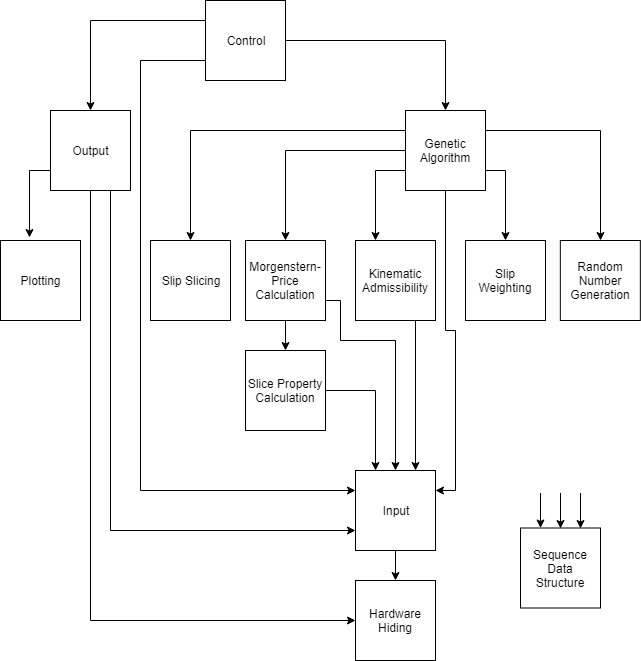
\includegraphics[width=1.1\textwidth]{UseHierarchyDiagram.png}
}
\caption{Use Hierarchy Diagram}
\label{Fig_Use}
\end{center}
\end{figure}
% ------ %
~\newpage
\bibliographystyle {plainnat}
\bibliography {../../../refs/References}

\end{document}
